\section{Χαρακτηριστικά που υλοποιήθηκαν} \label{section:4-5-implemented-parts}

Κατά την υλοποίηση εμφανίστηκαν διάφορα προβλήματα που δεν είχαν προβλεφθεί όπως αναλύθηκε στο προηγούμενο κεφάλαιο και τα οποία προκάλεσαν καθυστερήσεις στην ολοκλήρωση των tasks. Λόγω των καθυστερήσεων αυτών έγιναν διάφορες αναδιαμορφώσεις του προγραμματισμού των Sprint καθώς και διαπραγματεύσεις της σημαντικότητας των χαρακτηριστικών. Από τον επανασχεδιασμό και τις προσαρμογές αυτές προέκυψαν μερικές αλλαγές στο τελικό σετ των χαρακτηριστικών της πλατφόρμας σε σχέση με ό,τι είχε αρχικά προδιαγραφεί. Τα χαρακτηριστικά που υλοποιήθηκαν τελικά είναι:

\begin{itemize}
    \item η εγγραφή χρήστη και η δημιουργία των τοπικών βάσεων του όπως περιγράφεται στις \ref{srs:functional-srs-sign-up} \& \ref{srs:functional-srs-create-user-databases} και στο σενάριο χρήσης \ref{subsection:3-6-use-case-signup}
    \item η αυτόματη είσοδος χρήστη όπως περιγράφεται στην \ref{srs:functional-srs-sign-in} και στο σενάριο χρήσης \ref{subsection:3-6-use-case-signin}
    \item η δημιουργία θέματος και η δημιουργία ψηφοφοριών όπως περιγράφεται στις \ref{srs:functional-srs-create-topic} \& \ref{srs:functional-srs-create-polls} και στο σενάριο χρήσης \ref{subsection:3-6-use-case-create-topic}
    \item η περιήγηση στα υπάρχοντας θέματα όπως περιγράφεται στην \ref{srs:functional-srs-browse-topics} και στο σενάριο χρήσης \ref{subsection:3-6-use-case-fetch-topic}
    \item η δημοσίευση μηνύματος όπως περιγράφεται στην \ref{srs:functional-srs-create-post} και στο σενάριο χρήσης \ref{subsection:3-6-use-case-create-post}
    \item η επεξεργασία μηνύματος όπως περιγράφεται στην \ref{srs:functional-srs-modify-post} και στο σενάριο χρήσης \ref{subsection:3-6-use-case-modify-post}
    \item η ψήφιση σε ψηφοφορία όπως περιγράφεται στην \ref{srs:functional-srs-vote-polls} και στο σενάριο χρήσης \ref{subsection:3-6-use-case-vote-in-poll}
    \item η ψήφιση σε μηνύματα όπως περιγράφεται στην \ref{srs:functional-srs-vote-posts} και στο σενάριο χρήσης \ref{subsection:3-6-use-case-vote-post}
    \item η διαγραφή των τοπικών δεδομένων όπως περιγράφεται στην \ref{srs:functional-srs-delete-local-data} και στο σενάριο χρήσης \ref{subsection:3-6-use-case-delete-local-data}
\end{itemize}

Τα παραπάνω αντιστοιχούν σε 11 ολοκληρωμένες από τις 13 προδιαγεγραμμένες ΛΑ ή πλήρωση 84.6\%, ποσοστό που θεωρείται από τους συγγραφείς επαρκές για την εξαγωγή συμπερασμάτων για τον χώρο των DApps και υπερβάλλων για τα πλαίσια ενός PoC. Στο παράρτημα \ref{screenshots-appendix} παρατίθενται τα στιγμιότυπα οθόνης των υλοποιημένων χαρακτηριστικών.

Τα χαρακτηριστικά τα οποία παραλήφθηκαν είναι τα παρακάτω:

\begin{itemize}
    \item η δημιουργία κοινοτήτων και ο ορισμός εξωτερικών contracts για τα tokens τους όπως περιγράφεται στις \ref{srs:functional-srs-create-communities} \& \ref{srs:functional-srs-assign-community-contract} και στο σενάριο χρήσης \ref{subsection:3-10-use-case-create-community}
\end{itemize}

Τέλος, η ΜΛΑ που αφορά την ελαχιστοποίηση των fees (\ref{srs:non-functional-srs-minimize-fees}) ακολουθήθηκε κατά το δυνατόν σε όλη τη διαδικασία σχεδιασμού και υλοποίησης. Η ΜΛΑ σχετικά με την αναβαθμισιμότητα των contracts (\ref{srs:non-functional-srs-upgrade-contracts}) καταστρατηγήθηκε λόγω του χρόνου που θα απαιτούσε μία τέτοια υλοποίηση.

Η \ref{srs:non-functional-srs-maximum-decentraliztion} απαιτεί την μεγιστοποίηση της αποκέντρωσης της πλατφόρμας. Παρότι υπάρχουν μέρη τα οποία φαινομενικά έχει παραβιαστεί, όπως η διάθεση της εφαρμογής και των contract artifacts μέσω κεντροποιημένων servers καθώς και η ύπαρξη του rendezvous server, στην πραγματικότητα έχει ακολουθηθεί σε ικανοποιητικό βαθμό. Σχετικά με την εφαρμογή και τα contracts, πάρθηκε η απόφαση να διατεθούν μέσω των αντίστοιχων servers επειδή αυτό προσφέρει μεγάλη ευελιξία και ευκολία στην ανάπτυξη. Θα μπορούσαν εύκολα να διατεθούν μέσω αποκεντρωμένων συστημάτων όπως torrents ή το IPFS και αυτό παραμένει ένα ανοιχτό θέμα. Επίσης ανοιχτό θέμα παραμένει η ανάγκη ύπαρξης του rendezvous server. Λόγω της φύσης του πρωτοκόλλου IPFS και της λειτουργίας που επιτελεί ο server αυτός, είναι αδύνατον να παραληφθεί, ωστόσο είναι ανοιχτό ερευνητικό πεδίο η περαιτέρω αποκέντρωση του πρωτοκόλλου.
% https://mnot.github.io/avoiding-internet-centralization/draft-nottingham-avoiding-internet-centralization.html#name-necessary-centralization

\subsection{Διαφορές σχεδιασμού-υλοποίησης} \label{subsection:4-6-1-design-implementation-differences}

Σημαντικές διαφορές υπήρξαν επίσης στην διαδικασία υλοποίησης τόσο όσον αφορά τον αριθμό και τις λειτουργίες των διαφορετικών πακέτων λογισμικού όσο και τον χρονοπρογραμματισμό. Προστέθηκαν τρεις νέες υπηρεσίες, η υπηρεσία "Concordia Contracts Provider", ο προσαρμοσμένος IPFS pinner και η ιστοσελίδα "Concordia Guide".

Η ανάγκη για τα νέα πακέτα λογισμικού προέκυψε κατά την πορεία υλοποίησης της διπλωματικής και προστέθηκαν στον χρονοπρογραμματισμό που είχε γίνει στην αρχή της εργασίας. Στην προσαρμογή αυτή βοήθησαν ιδιαίτερα οι Agile τακτικές που ακολουθήθηκαν και η προσαρμοστικότητα που προσφέρει το Scrum σε μεταβαλλόμενες απαιτήσεις.

Τέλος, κατά την υλοποίηση έγινε γρήγορα αντιληπτή η αξία που προσφέρουν ένα δοκιμαστικό περιβάλλον (staging environment) σε συνδυασμό με ένα CI/CD σύστημα. Για το λόγο αυτό πάρθηκε η απόφαση να μεταφερθεί το sprint που αφορούσε αυτά πολύ νωρίτερα στην διαδικασία υλοποίησης, ώστε να μεγιστοποιηθεί η χρήση του.

Εποπτικά, η διαδικασία της υλοποίησης περιγράφεται στο παρακάτω σχήμα (σχήμα \ref{figure:4.6.design-implementation-differences-sprints}). Με σκούρο πράσινο χρώμα εμφανίζονται τα tasks τα οποία υπήρχαν στο χρονοπρογραμματισμό από τη αρχή και υλοποιήθηκαν, με ανοιχτό πράσινο αυτά τα οποία δεν υπήρχαν στον αρχικό προγραμματισμό αλλά υλοποιήθηκαν και με κόκκινο αυτά τα οποία δεν υλοποιήθηκαν.

\begin{figure}[H]
    \centering
    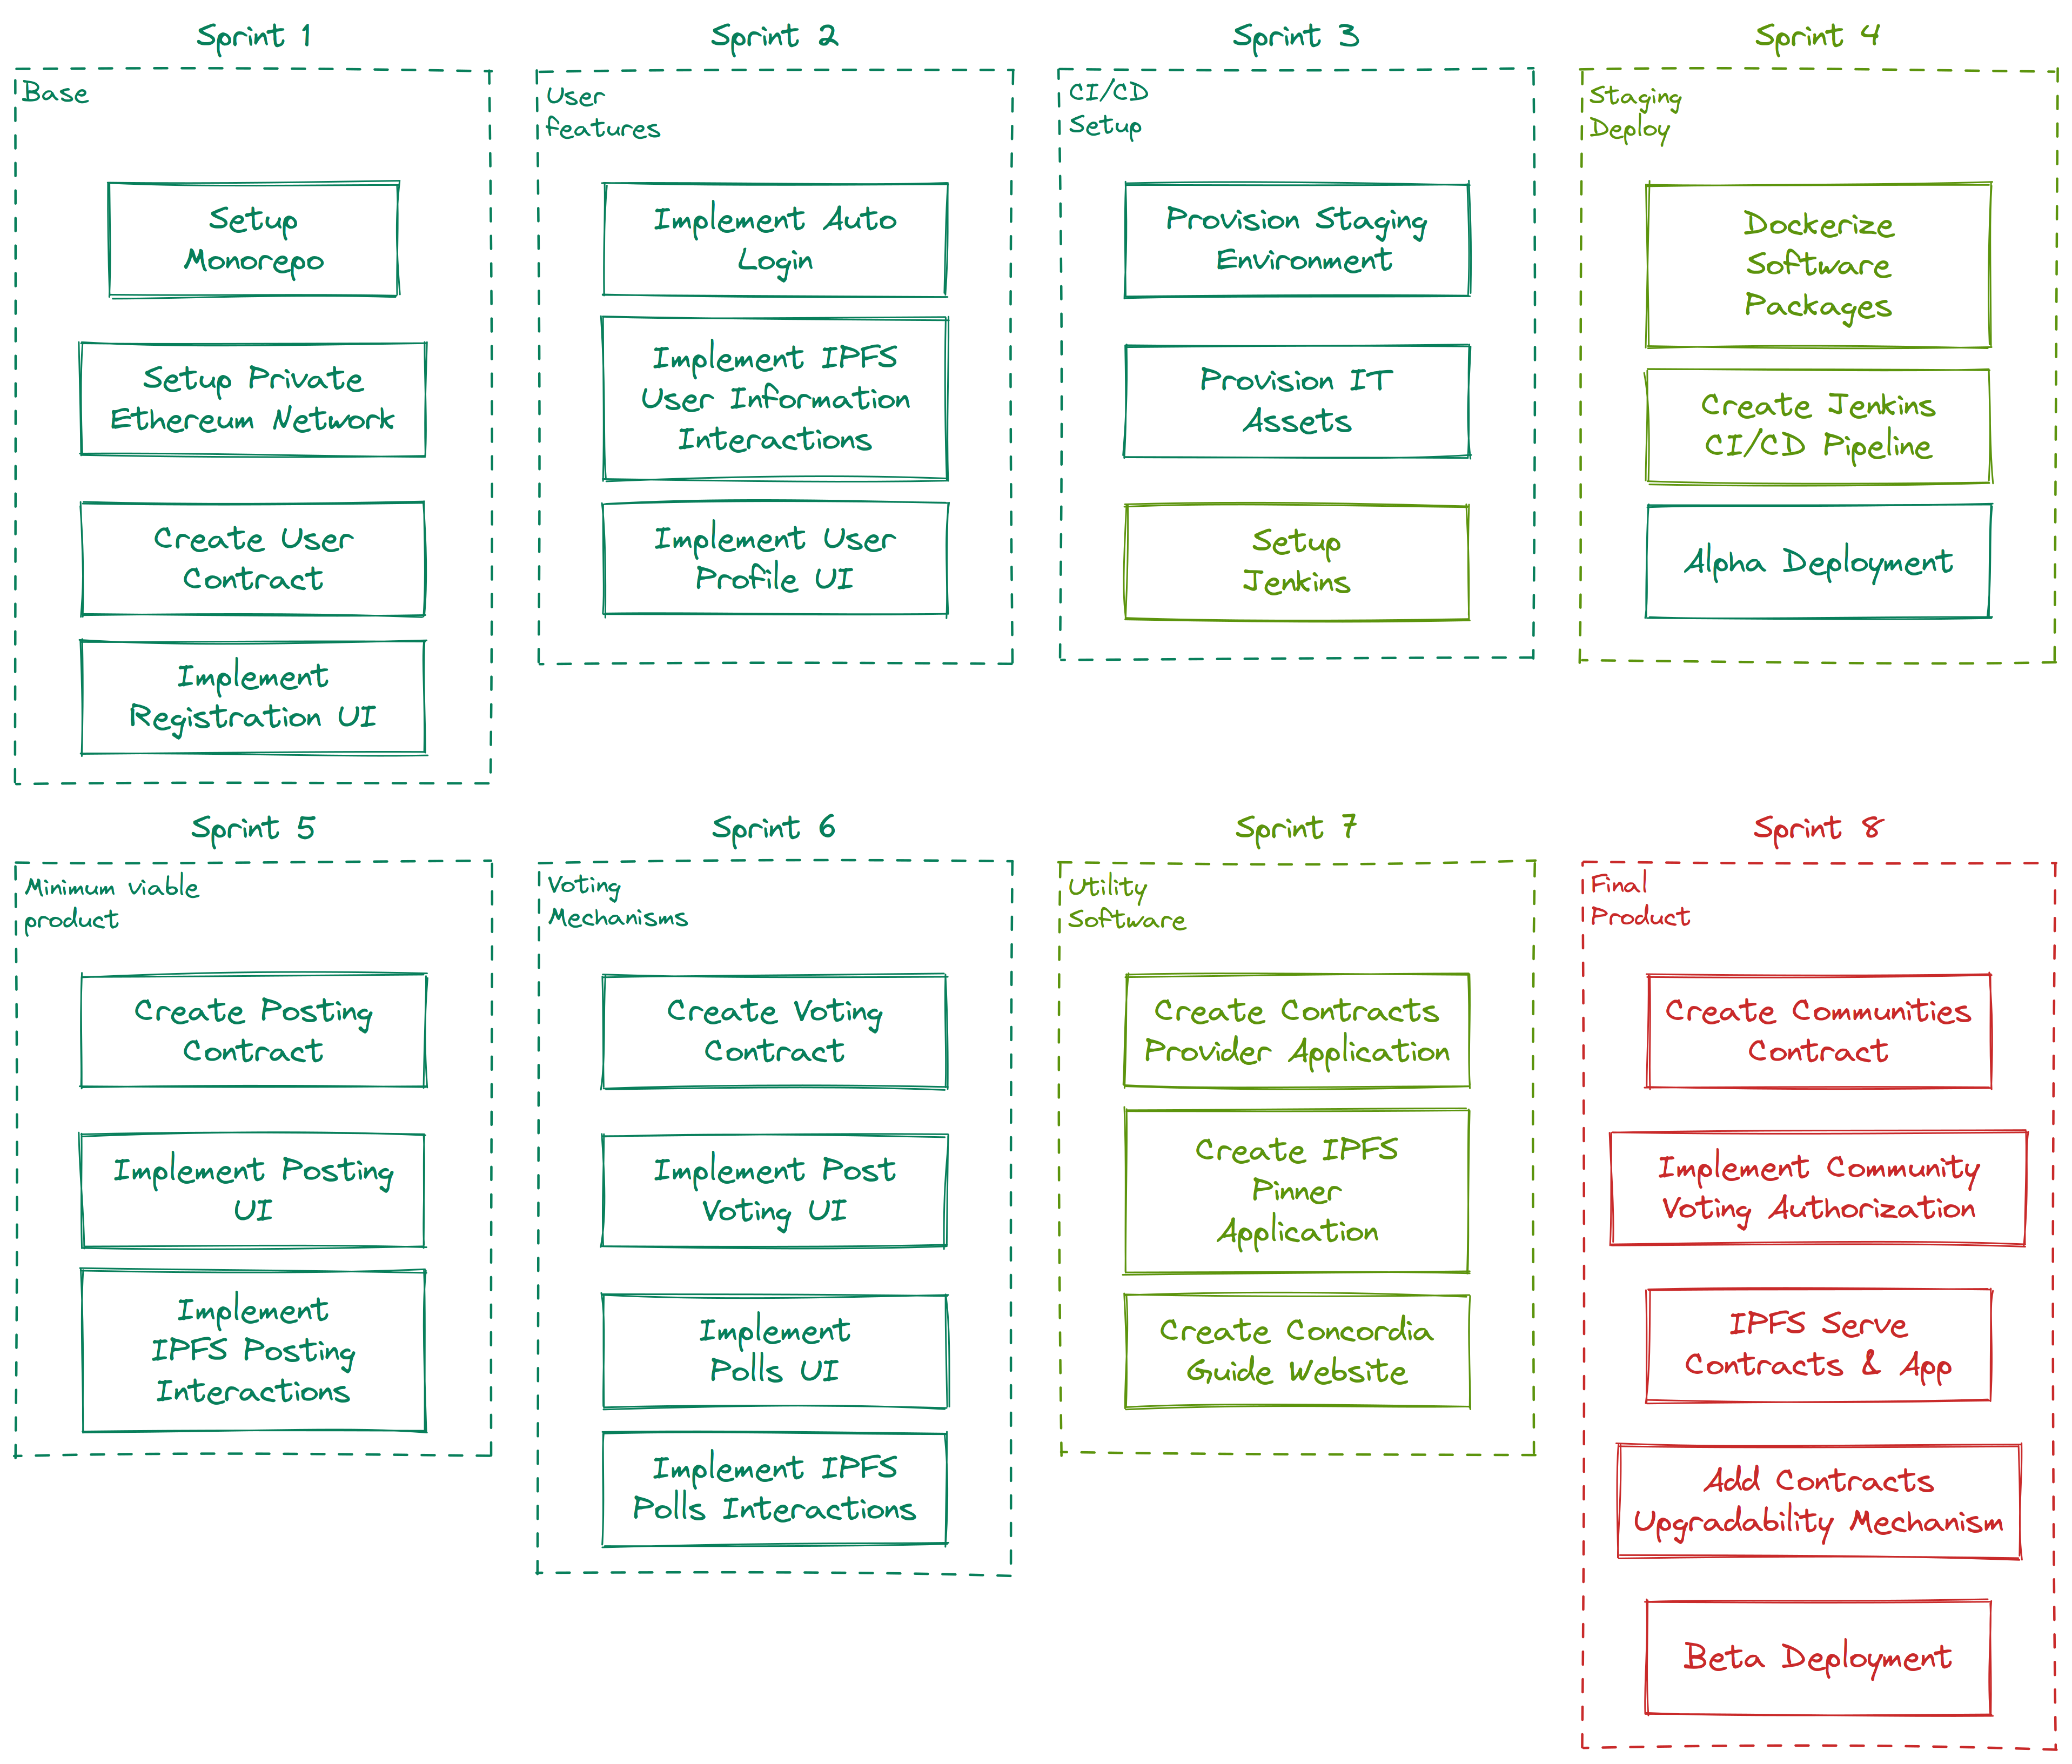
\includegraphics[width=\textwidth]{assets/figures/chapter-4/4.6.design-implementation-differences-sprints.png}
    \caption{Διαχωρισμός σε sprints}
    \label{figure:4.6.design-implementation-differences-sprints}
\end{figure}
